\documentclass[]{book}
\usepackage{lmodern}
\usepackage{amssymb,amsmath}
\usepackage{ifxetex,ifluatex}
\usepackage{fixltx2e} % provides \textsubscript
\ifnum 0\ifxetex 1\fi\ifluatex 1\fi=0 % if pdftex
  \usepackage[T1]{fontenc}
  \usepackage[utf8]{inputenc}
\else % if luatex or xelatex
  \ifxetex
    \usepackage{mathspec}
  \else
    \usepackage{fontspec}
  \fi
  \defaultfontfeatures{Ligatures=TeX,Scale=MatchLowercase}
\fi
% use upquote if available, for straight quotes in verbatim environments
\IfFileExists{upquote.sty}{\usepackage{upquote}}{}
% use microtype if available
\IfFileExists{microtype.sty}{%
\usepackage{microtype}
\UseMicrotypeSet[protrusion]{basicmath} % disable protrusion for tt fonts
}{}
\usepackage[margin=1in]{geometry}
\usepackage{hyperref}
\hypersetup{unicode=true,
            pdftitle={Guide d'organisation d'un data sprint},
            pdfauthor={Samuel Goëta (Datactivist) pour le lab 110bis du ministère de l'Éducation nationale},
            pdfborder={0 0 0},
            breaklinks=true}
\urlstyle{same}  % don't use monospace font for urls
\usepackage{natbib}
\bibliographystyle{apalike}
\usepackage{longtable,booktabs}
\usepackage{graphicx,grffile}
\makeatletter
\def\maxwidth{\ifdim\Gin@nat@width>\linewidth\linewidth\else\Gin@nat@width\fi}
\def\maxheight{\ifdim\Gin@nat@height>\textheight\textheight\else\Gin@nat@height\fi}
\makeatother
% Scale images if necessary, so that they will not overflow the page
% margins by default, and it is still possible to overwrite the defaults
% using explicit options in \includegraphics[width, height, ...]{}
\setkeys{Gin}{width=\maxwidth,height=\maxheight,keepaspectratio}
\IfFileExists{parskip.sty}{%
\usepackage{parskip}
}{% else
\setlength{\parindent}{0pt}
\setlength{\parskip}{6pt plus 2pt minus 1pt}
}
\setlength{\emergencystretch}{3em}  % prevent overfull lines
\providecommand{\tightlist}{%
  \setlength{\itemsep}{0pt}\setlength{\parskip}{0pt}}
\setcounter{secnumdepth}{5}
% Redefines (sub)paragraphs to behave more like sections
\ifx\paragraph\undefined\else
\let\oldparagraph\paragraph
\renewcommand{\paragraph}[1]{\oldparagraph{#1}\mbox{}}
\fi
\ifx\subparagraph\undefined\else
\let\oldsubparagraph\subparagraph
\renewcommand{\subparagraph}[1]{\oldsubparagraph{#1}\mbox{}}
\fi

%%% Use protect on footnotes to avoid problems with footnotes in titles
\let\rmarkdownfootnote\footnote%
\def\footnote{\protect\rmarkdownfootnote}

%%% Change title format to be more compact
\usepackage{titling}

% Create subtitle command for use in maketitle
\providecommand{\subtitle}[1]{
  \posttitle{
    \begin{center}\large#1\end{center}
    }
}

\setlength{\droptitle}{-2em}

  \title{Guide d'organisation d'un data sprint}
    \pretitle{\vspace{\droptitle}\centering\huge}
  \posttitle{\par}
    \author{Samuel Goëta (Datactivist) pour le lab 110bis du ministère de
l'Éducation nationale}
    \preauthor{\centering\large\emph}
  \postauthor{\par}
      \predate{\centering\large\emph}
  \postdate{\par}
    \date{2019-04-18}

\usepackage{booktabs}

\begin{document}
\maketitle

{
\setcounter{tocdepth}{1}
\tableofcontents
}
\chapter{Introduction}\label{introduction}

A la suite du dataviz challenge organisé les 22 et 23 mars 2019, le
guide d'organisation d'un data sprint doit : * Permettre l'essaimage du
format au sein du Ministère de l'Education nationale et de la Jeunesse
et auprès de ses partenaires ainsi que dans les territoires * Rendre
l'évènement réplicable * Restituer l'expérience du dataviz challenge et
inciter d'autres acteurs à le reproduire.

Le guide est open source, il s'appuie sur le
\href{https://docs.google.com/document/d/1uDw4Maifjl_egJ95y-F0dkXEyu2MNfhc2GvNEmjhPq8/edit\#heading=h.9ofnjz67swln}{travail
réalisé par Datactivist pour le département de l'Ardèche} sous licence
\href{https://creativecommons.org/licenses/by-sa/4.0/deed.fr}{CC BY-SA
4.0} (Attribution - Partage dans les Mêmes Conditions 4.0
International). Le guide est publié avec la même licence qui permet la
libre réutilisation tout en garantissant que le contenu restera ouvert.

Pour favoriser la réplication de l'évènement, le guide comprend des
conseils méthodologiques ainsi que des documents type qui faciliteront
l'organisation de ce type d'évènements.

\chapter{Le dataviz challenge : un évènement à répliquer}\label{dataviz}

Le dataviz challenge s'est inscrit dans le cadre de la mission relative
aux politiques éducatives territoriales confiée en octobre 2018 par le
ministre de l'Education nationale et de la Jeunesse, Jean-Michel
Blanquer, à Ariane Azéma, inspectrice générale de l'administration de
l'éducation nationale et de la recherche et à Pierre Mathiot, professeur
des universités.

Il part du constat que la concentration géographique des inégalités
sociales et ses effets sur l'échec scolaire est identifiée depuis de
nombreuses années en France : elle est un des fondements historiques des
politiques d'éducation prioritaire. Le ministère doit procéder à la
révision de la carte de la géographie prioritaire et veut, plus
globalement, mieux prendre en compte l'ensemble des enjeux territoriaux
qui contribuent à la réussite de tous les élèves.

Dans le cadre de cette mission, le
\href{https://www.education.gouv.fr/110bislab/cid130754/presentation-du-110-bis-lab-d-innovation-de-l-education-nationale.html}{110
bis}, lab d'innovation de l'Education nationale, a expérimenté du
vendredi 22 mars 9h au samedi 23 mars 19h un nouveau format
d'exploitation de données visant à co-construire des outils, une
méthodologie et des pratiques pour améliorer les politiques publiques
éducatives.

L'évènement s'adressait à un large public : développeur, enseignant,
data scientist, designer, chercheur, professionnel de l'éducation,
décideur public, étudiant, et quiconque souhaitant apporter sa
contribution sur le sujet des politiques éducatives territoriales et
s'immerger dans une équipe interdisciplinaire le temps des deux jours du
dataviz challenge.

\begin{figure}

{\centering 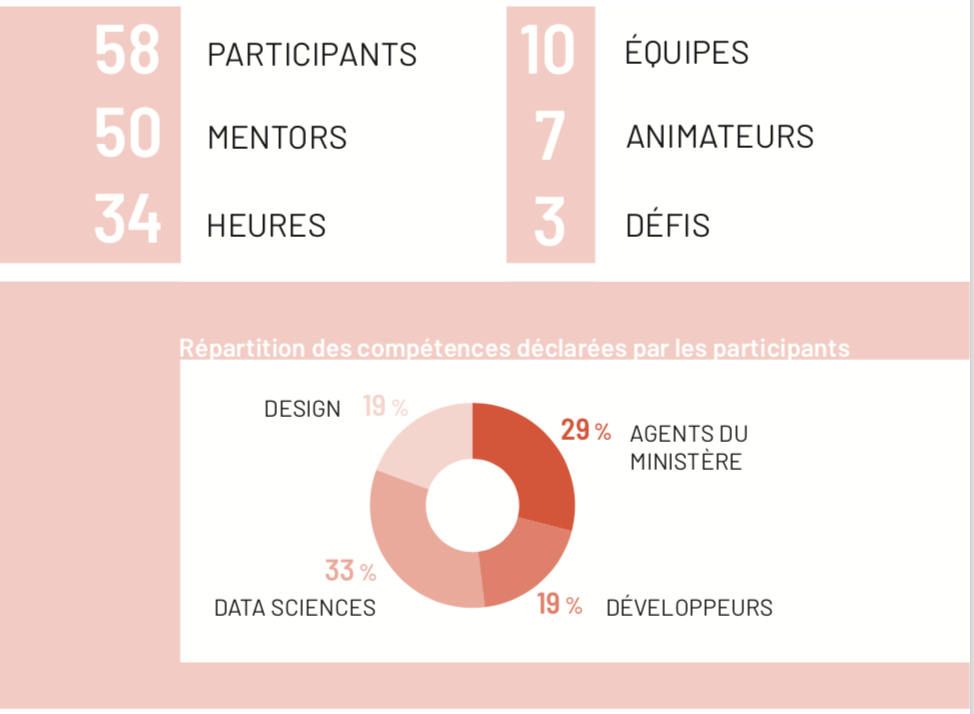
\includegraphics[width=0.5\linewidth]{./img/participants} 

}

\caption{Extrait du livret du dataviz challenge représentant la diversité des participants}\label{fig:unnamed-chunk-1}
\end{figure}

Les 3 défis du dataviz challenge ont été identifiés lors d'une journée
contributive le 3 octobre 2018 avec les acteurs de terrain.

Les défis 1 et 2 se sont appuyés sur des données qui ne sont pas
librement réutilisables en open data. Bien qu'anonymisées, ces données
concernaient des personnes physiques ou morales et les participants se
sont engagés à ne pas ni altérer les données, ni dénaturer leur sens et
à présenter les résultats de manière à ne pas permettre une éventuelle
identification.

\section{Défi 1 : «Les déplacements en
cascade»}\label{defi-1-les-deplacements-en-cascade}

\subsection{Cadrage du défi}\label{cadrage-du-defi}

L'émergence des campus des métiers et des qualifications, le
développement de l'apprentissage, la réforme du lycée, etc. sont autant
de politiques publiques éducatives qui peuvent se traduire par la
modification de l'offre de formation sur le territoire. Comment
représenter les conséquences potentielles de ces modifications sur les
déplacements des élèves et des professeurs ?

\textbf{Objectifs} : anticiper les impacts plausibles d'une modification
de l'offre de formation au niveau local, sur les déplacements des
professeurs et des élèves (nombre de personnes impactées, temps de
transport, etc.)

\textbf{3 questions pour démarrer le DataViz Challenge :}

\begin{itemize}
\item
  Comment mettre en regard le déplacement de l'offre de formation et
  l'offre de transports, dont une partie est gérée par les collectivités
  ?
\item
  Comment tenir compte et représenter les différentes stratégies qui
  peuvent être mises en oeuvre par les élèves ?
\item
  Quels sont les effets du déplacement d'une option ou d'une spécialité
  sur la mixité sociale ?
\end{itemize}

3 projets ont été développés dans le cadre de ce défi.

\subsection{\texorpdfstring{🏆 Projet ``Mixité
Sociale''}{🏆 Projet Mixité Sociale}}\label{projet-mixite-sociale}

\begin{quote}
\emph{Ce projet a été retenu par le jury pour le défi 1.} Lien vers le
code et la documentation : \url{https://github.com/kir0ul/DataTerr}
\end{quote}

\textbf{Contexte}

Au sein d'un périmètre restreint, des établissements peuvent être
caractérisés par des niveaux de mixité sociale, entendue comme la
représentation équilibrée de toutes les différentes professions et
catégories socioprofessionnelles (PCS), très inégaux.

A Bordeaux, trois collèges publics limitrophes ont des indices de mixité
respectifs de 30,4, 46,2 et 9,7 \%, tandis que la moyenne académique est
de 34,9\%.

Comment améliorer cet indice, notamment pour les établissements où il
demeure faible ? Comment identifier les variables sur lesquelles jouer
et leur impact plausible sur l'indice de mixité d'établissements proches
?

\textbf{Produit final} S'appuyant sur QGIS pour explorer les données,
l'équipe s'est focalisée sur la ville de Bordeaux car nous disposions
des données de carte scolaire. Chaque établissement est représenté par
ses indicateurs PCS, le nombre d'élève de secteur non présent dans
l'établissement, l'indicateur PCS\_D (catégories sociaux
professionnelles défavorisées) prédit par le modèle, et enfin
l'indicateur PCS\_D après déplacement d'options.

L'équipe avait aussi pour projet de développer également une aide à la
modification des cartes scolaires, non réalisée faute de temps.

\begin{figure}

{\centering 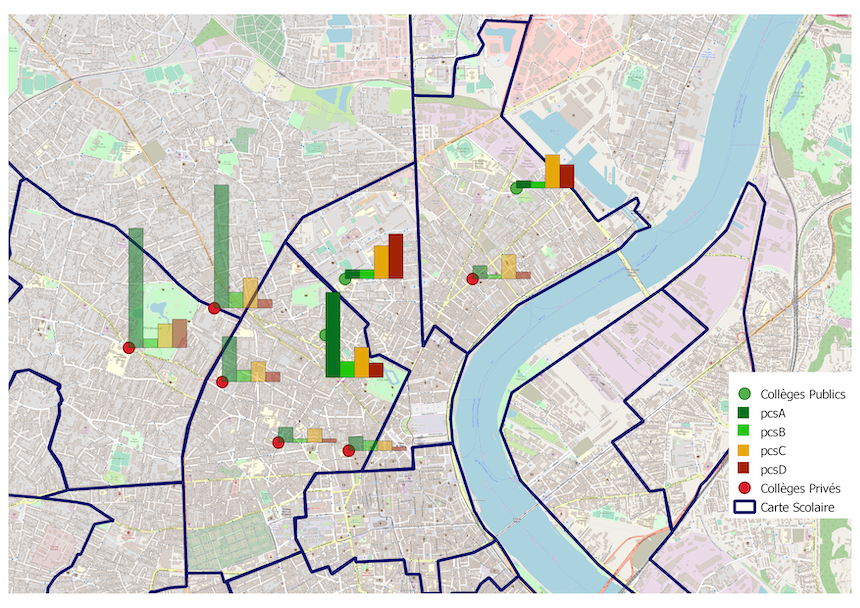
\includegraphics[width=0.6\linewidth]{./img/Diagramme_Publics_Prives} 

}

\caption{Exemple de carte prédisantle  niveau de mixité sociale}\label{fig:unnamed-chunk-2}
\end{figure}

\textbf{Méthode} Le modèle choisi est un
\href{https://fr.wikipedia.org/wiki/For\%C3\%AAt_d\%27arbres_d\%C3\%A9cisionnels}{régresseur
à base de forêts aléatoires}. La variable à prédire est le taux d'élèves
en PCS très défavorisé et les variables d'entrée sont le nombre
d'élèves, secteur/privé, le nombre d'options disponibles, et les options
d'intérêt.

\begin{figure}

{\centering 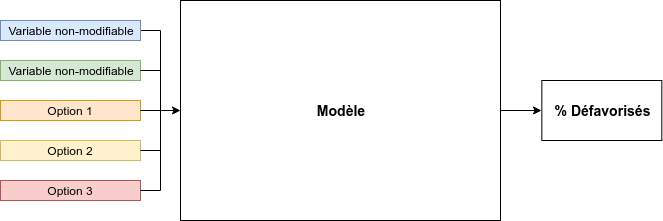
\includegraphics[width=0.6\linewidth]{./img/model-diag} 

}

\caption{Représentation synthétique du modèle}\label{fig:unnamed-chunk-3}
\end{figure}

Malgré la simplicité de cette sélection de variables, le modèle a une
\href{https://fr.wikipedia.org/wiki/Erreur_quadratique_moyenne}{erreur
RMSE}, mesure caractérisant la « précision » d'un estimateur, de 2\% ce
qui est très faible.

\begin{figure}

{\centering 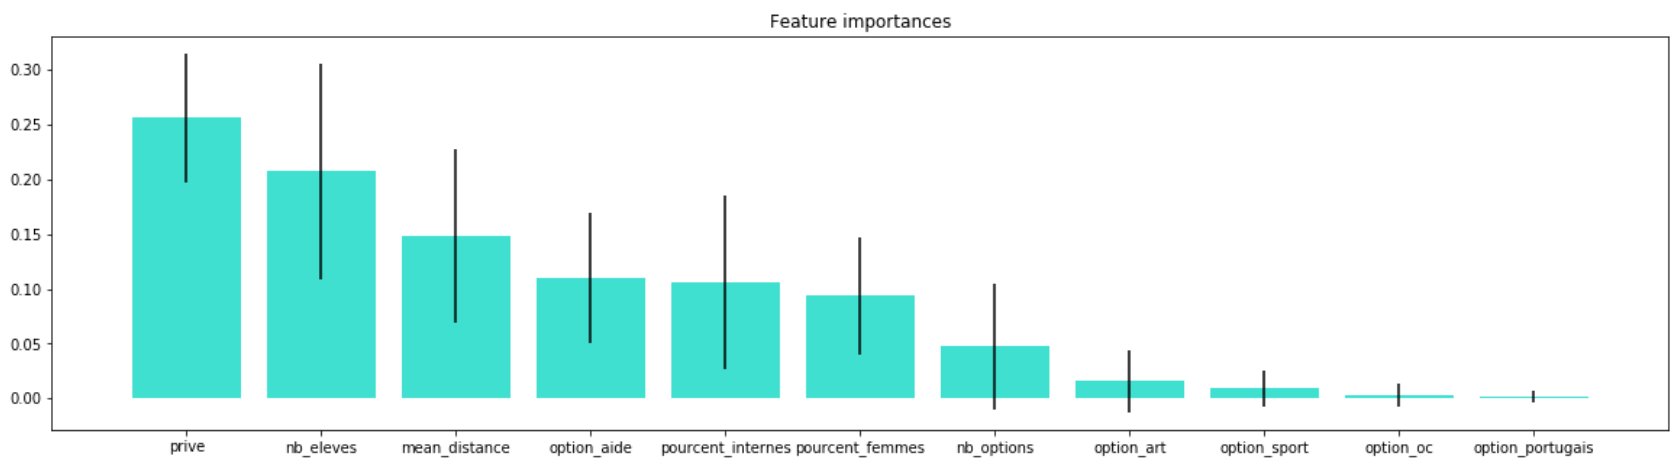
\includegraphics[width=1\linewidth]{./img/model-vars} 

}

\caption{Représentation sous forme de boite à moustache de la hiérarchisation automatique des variables utilisées par le modèle}\label{fig:unnamed-chunk-4}
\end{figure}

\subsection{\texorpdfstring{Projet
``Locaviz''}{Projet Locaviz}}\label{projet-locaviz}

\begin{quote}
\href{https://drive.google.com/file/d/1gpl02y7FG4hOCEh2t55YRlaRyTP010Pj/view?usp=sharing}{Lien
vers le code et la documentation du projet}
\end{quote}

\textbf{Contexte :} La fermeture ou l'ouverture d'un établissement
scolaire peut avoir de sérieux impacts sur les capacités d'accueil des
établissements similaires voisins, trajets quotidiens des élèves, et
donc sur des enjeux plus vastes tels que l'environnement.

Comment prévoir les impacts de la fermeture ou de l'ouverture d'un
établissement sur ces trois paramètres ?

\textbf{Produit final}: Une carte décrivant les impacts de la fermeture
d'un établissement sélectionné. En fonction du nombre de classes de
l'établissement, le prototype anticipe la réaffectation des élèves dans
les établissements environnants, ses impacts sur les trajets. Les
caractéristiques sociales de chaque établissement sont visualisées dans
une rosace qui se déplie par niveau.

\begin{figure}

{\centering 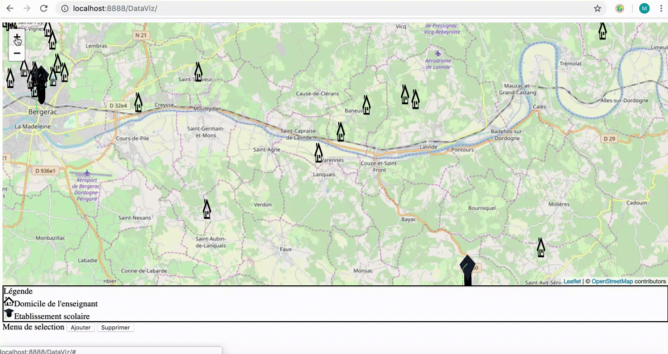
\includegraphics[width=0.6\linewidth]{./img/locaviz} 

}

\caption{Représentation cartographique de la suppression de la classe et des déplacements engendrés}\label{fig:unnamed-chunk-5}
\end{figure}

Le projet prévoit la réaffectation des élèves dans les établissements en
prenant en compte sa capacité actuelle et sa capacité après
réaffectation. Le temps de trajet n'a pu être calculé mais la distance
est représentée avec une estimation de l'impact carbone de ces
déplacements.

\subsection{Projet I.P.E.D. (Indice de Performance des
Déplacements)}\label{projet-i.p.e.d.-indice-de-performance-des-deplacements}

\begin{quote}
\href{http://datavizchallenge.fr/t/defi-numero-1-indice-annuel-d-evaluation-de-l-impact-mobilite-des-enseignants/131}{Lien
vers le code et la documentation}
\end{quote}

\textbf{Contexte} : Les enseignants qui exercent au sein de plusieurs
établissements, ou enseignants en compléments de services, doivent
souvent assumer de nombreux déplacements qui peuvent sensiblement peser
sur leur vie personnelle et professionnelle. A terme, cela peut avoir
des impacts notoires sur d'autres paramètres tels que l'environnement ou
les chances de réussite des élèves.

Comment analyser ces déplacements pour apporter des solutions efficaces
permettant de les limiter et d'en réduire les impacts?

\begin{figure}

{\centering 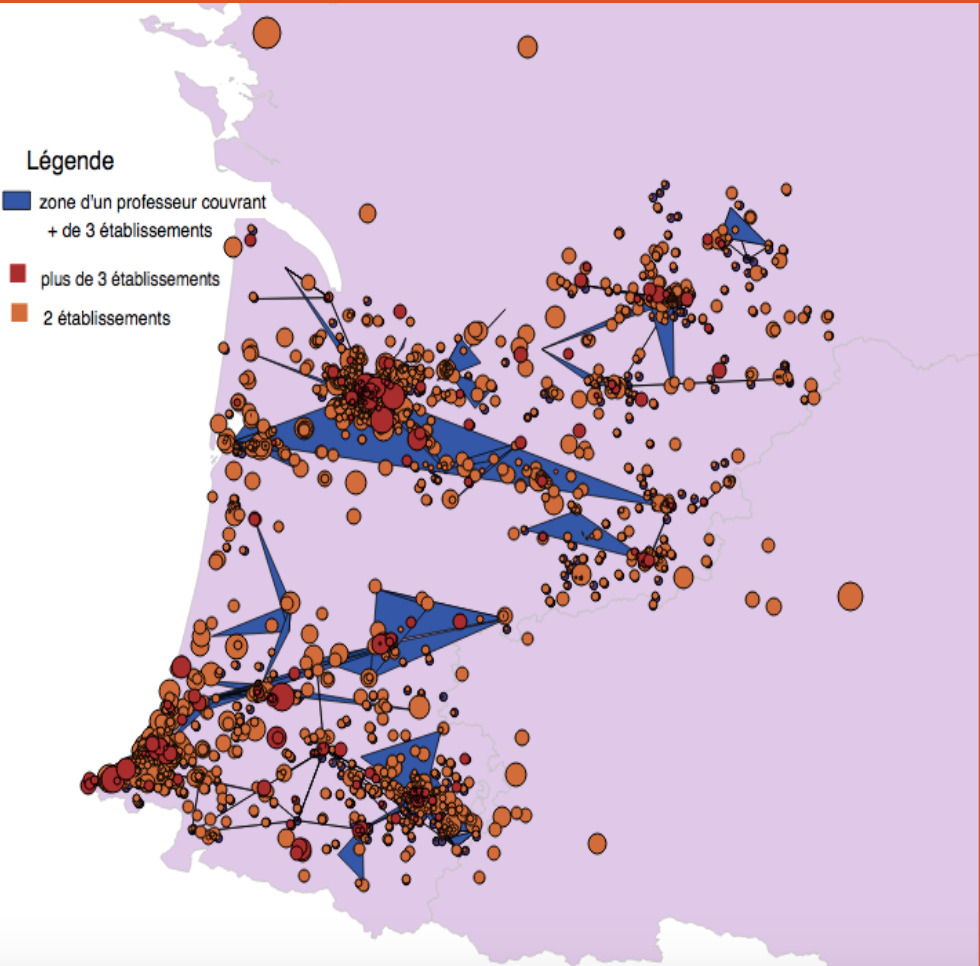
\includegraphics[width=0.6\linewidth]{./img/iped} 

}

\caption{Carte représentant les déplacements effectués par les enseignements en complément de service.}\label{fig:unnamed-chunk-6}
\end{figure}

\textbf{Produit Final} : Maquette de plateforme permettant de visualiser
l'évolution d'un Indice de Performance des Déplacements (IPED) en
fonction de l'évolution de paramètres qui déterminent l'offre éducative.

\begin{figure}

{\centering 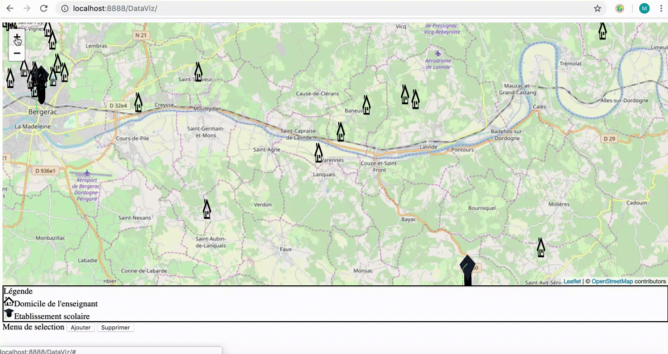
\includegraphics[width=0.6\linewidth]{./img/iped2} 

}

\caption{Maquette de la plateforme IPED.}\label{fig:unnamed-chunk-7}
\end{figure}

\textbf{Méthode} : Le projet a abouti à la création d'un indicateur IPED
:indice annuel, de base 100, d'évaluation de l'impact mobilité des
enseignants. Il se compose de l'addition globale des trajets à vol
d'oiseau de chacun.e des enseignant.e.s.

Selon le Lieu de résidence de l'enseignant, les matières et options
enseignées et la typologie de l'établissement, un algorithme recommande
un scénario d'optimisation des trajets.

\section{Défi 2 : la carte d'identité des établissements en temps
réel}\label{defi-2-la-carte-didentite-des-etablissements-en-temps-reel}

\subsection{Cadrage du défi}\label{cadrage-du-defi-1}

Les recteurs comme d'autres acteurs de l'Education nationale ont souvent
besoin de pouvoir prendre connaissance, en un coup d'oeil, de la
situation globale d'un établissement : l'état des ressources humaines et
financières, la situation sociale, les résultats des élèves, etc.
Comment remplacer une pile de dossiers papiers hétérogènes qui demandent
un effort considérable de constitution et de consultation, par une
vision synthétique, actualisée et à 360°, des informations relatives à
un établissement ?

\textbf{Objectifs} : avoir une vision consolidée et à jour d'un
établissement, diminuer le temps de préparation au profit du temps
consacré à l'échange, et ainsi faciliter le dialogue.

\textbf{3 questions pour démarrer le DataViz Challenge :}

\begin{itemize}
\tightlist
\item
  Comment synthétiser les informations nécessaires à la prise de
  connaissance de l'état d'un établissement ?
\item
  Comment permettre aux utilisateurs en mobilité (ex : recteurs) d'en
  disposer lors de leurs déplacements ?
\item
  Comment rendre cet outil utile pour des utilisateurs non experts de la
  donnée ?
\end{itemize}

\subsection{🏆Projet Eduscope}\label{projet-eduscope}

\begin{quote}
\emph{Ce projet a été retenu par le jury pour le défi 2.} Lien vers
l'outil : \url{https://avouacr.shinyapps.io/eduscope_shinyapp} Lien vers
le code et la documentation : \url{https://github.com/avouacr/EduScope}
\end{quote}

\textbf{Contexte} : Les recteurs, agents du ministère ou chefs
d'établissement ont souvent besoin d'obtenir rapidement des informations
sur les caractéristiques générales et les spécificités d'un
établissement cible. Aujourd'hui ces informations se trouvent dispersées
et stockées dans différentes bases de données (ex: GAIA, Mosart,
EPI\ldots{}), ce qui limite leur accessibilité, leur lisibilité et peut
donc complexifier la prise de décision.

Quel outil pourrait donc répondre aux besoins des différents
utilisateurs que sont: la visualisation rapide d'indicateurs, la
mobiquité et l'aide à la prise de décisions ?

\textbf{Produit final} : Plateforme interactive qui permet de
centraliser et de visualiser divers indicateurs de performance scolaire.
La priorisation des indicateurs d'intérêt s'adapte en fonction du profil
utilisateur (recteur, chef d'établissement, service support\ldots{}) et
de l'échelle de prise de décision souhaitée (nationale, académique,
département, bassin, établissement), tout en demeurant flexible.

\begin{figure}

{\centering 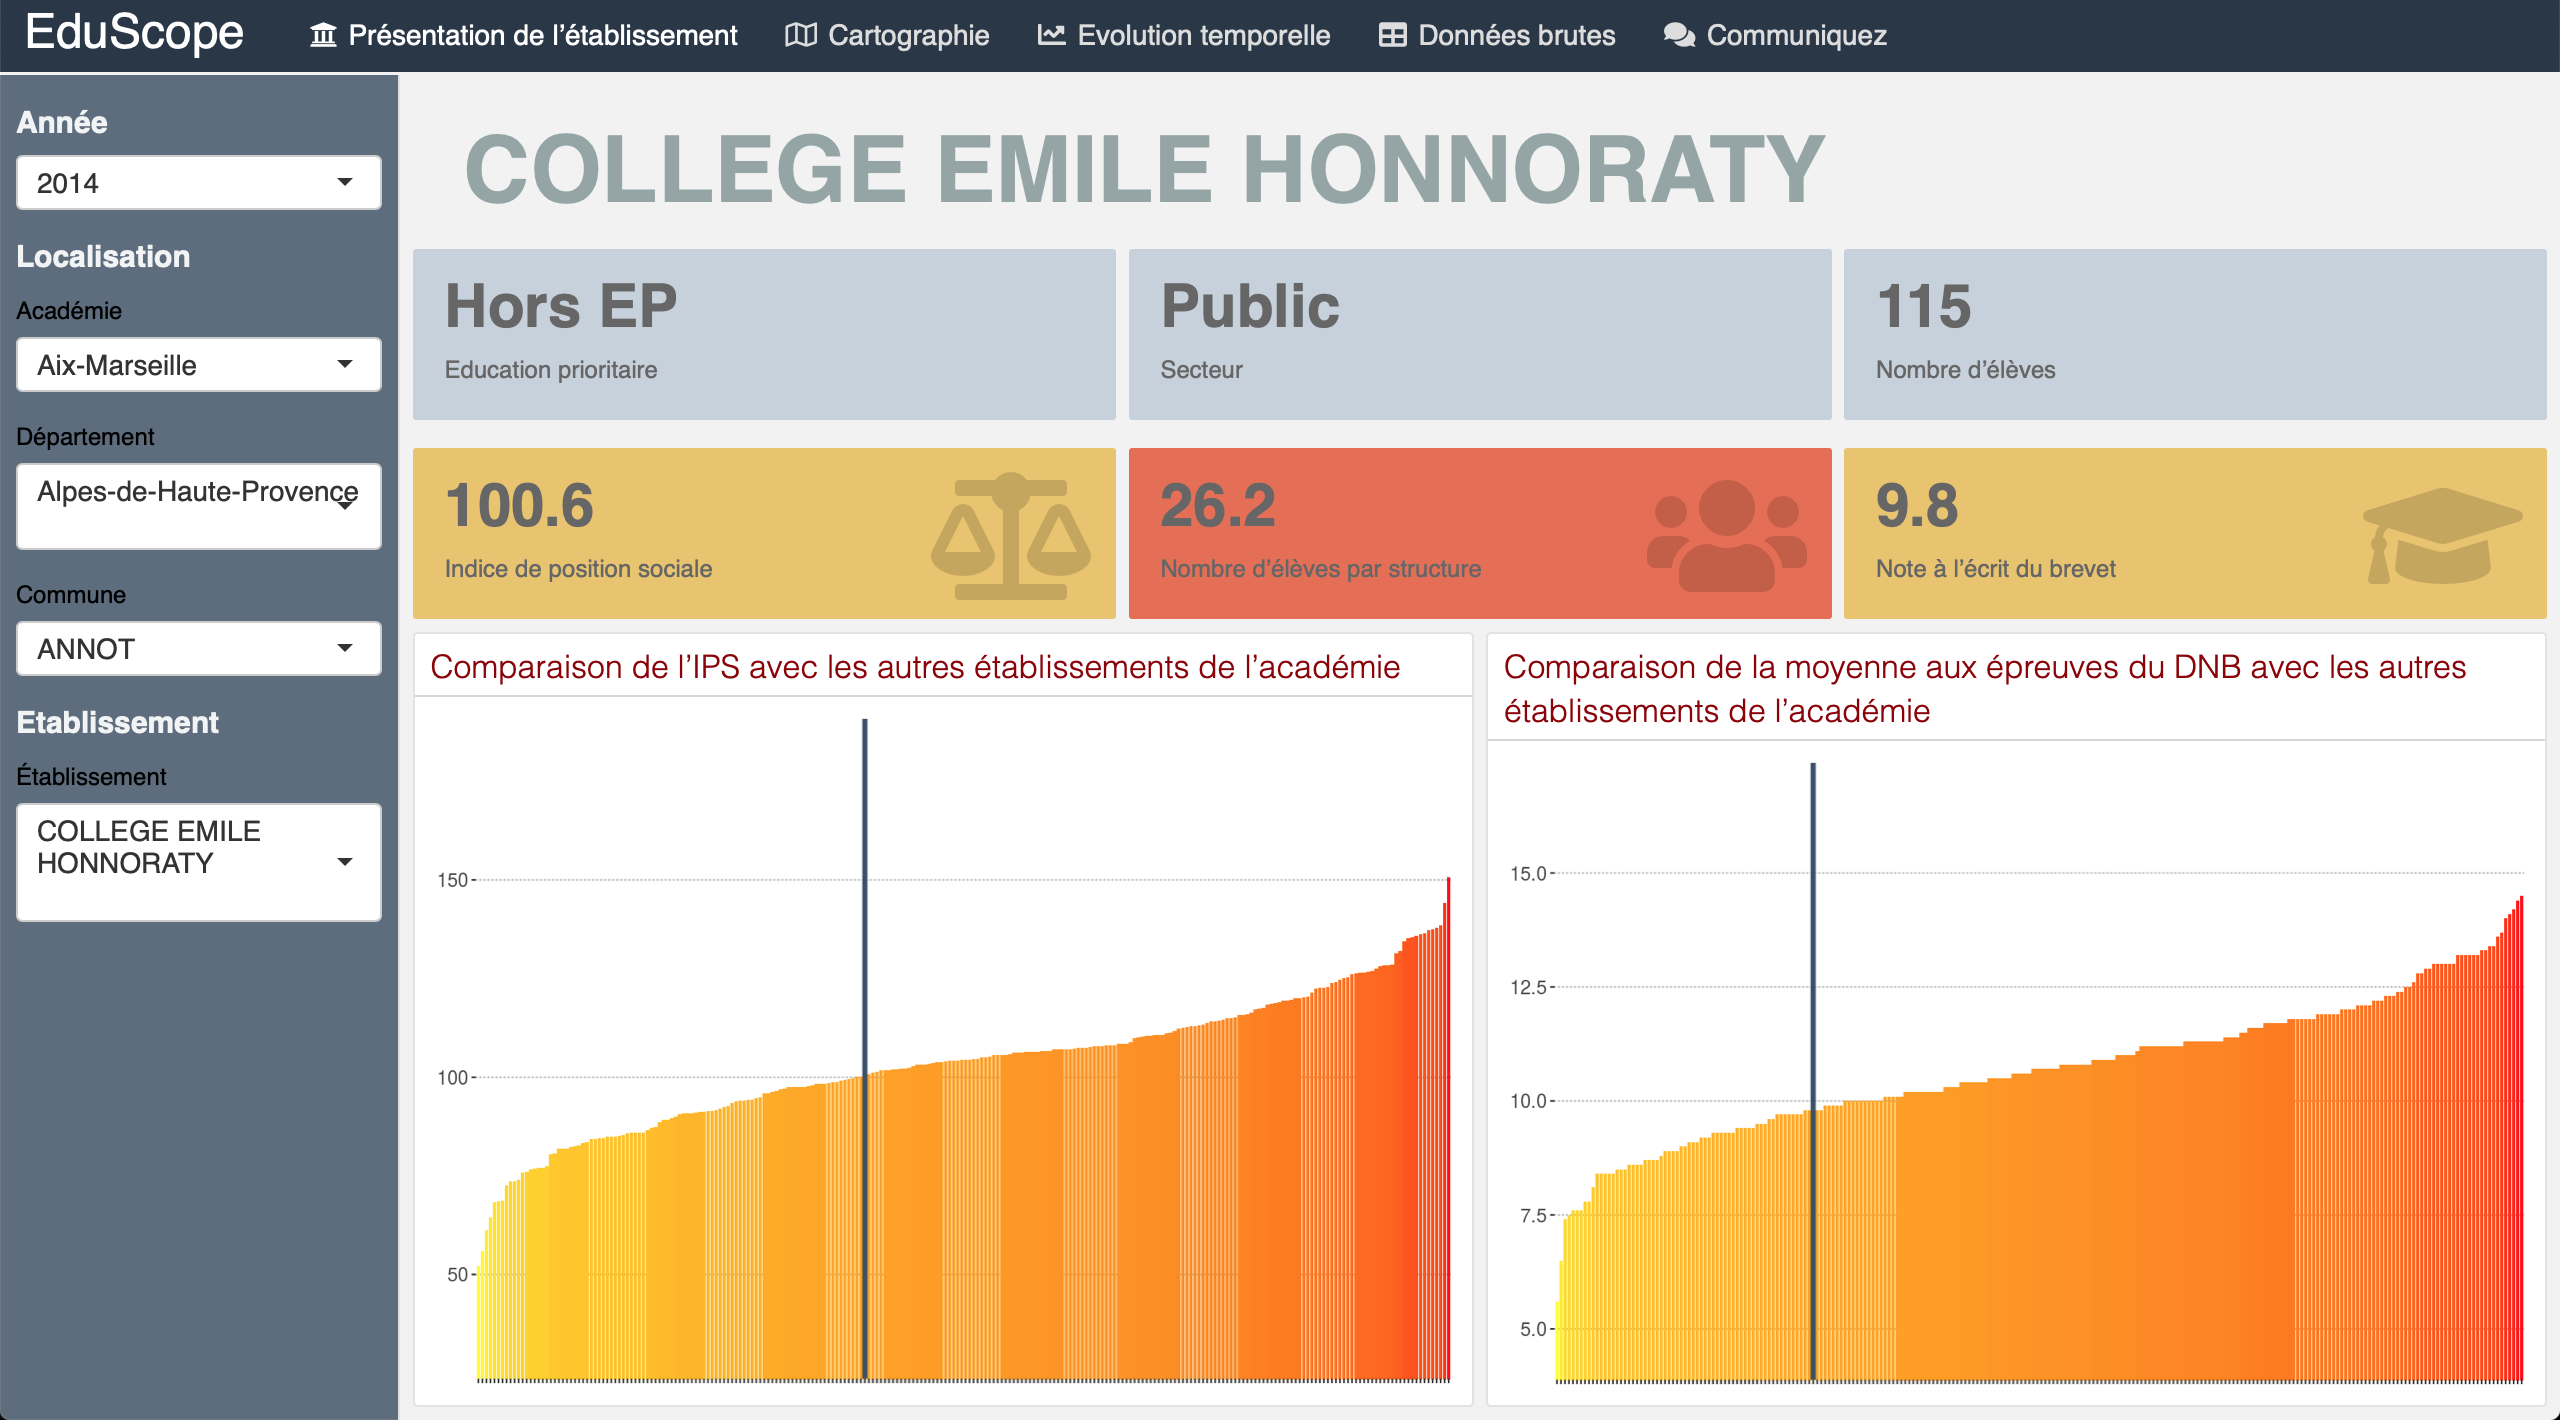
\includegraphics[width=0.6\linewidth]{./img/eduscope} 

}

\caption{Vue synthétique des données disponibles par établissement.}\label{fig:unnamed-chunk-8}
\end{figure}

La plateforme permet également de visualiser l'évolution des différents
indicateurs dans le temps, mais aussi de faire circuler des informations
qualitatives entre utilisateurs.

\subsection{Open}\label{open}

\begin{quote}
\href{http://datavizchallenge.fr/t/defi-n-2-open-placer-la-data-et-les-eleves-au-du-processus-de-decision/89/6}{Lien
vers la documentation}
\end{quote}

\textbf{Contexte} : L'identité d'un établissement se résume souvent à
bien plus que ses indicateurs de performance. Elle peut aussi être
enrichie par son dynamisme interne et son écosystème socio-culturel
(proximité des lieux culturels, des infrastructures sportives,
d'associations, etc). Ces informations peuvent être particulièrement
utiles pour les élèves, qui disposent actuellement de peu d'outils pour
comprendre et prendre part à la vie de leur établissement et tirer
profit de son environnement.

Comment remettre les élèves au centre de l'identité et du processus de
décision des établissements ?

\textbf{Produit final} : Maquette de plateforme participative accessible
aux élèves pourvus d'un identifiant. Elle leur donne la possibilité de
réagir, partager leur ressenti, mais aussi d'émettre des propositions
pour améliorer la vie dans leur établissement.

Elle propose également une vision géolocalisée de l'établissement
permettant aux élèves d'identifier les offres pédagogiques, sportives et
culturelles à proximité, puis d'effectuer un retour d'expérience sur ces
offres.

\begin{figure}

{\centering 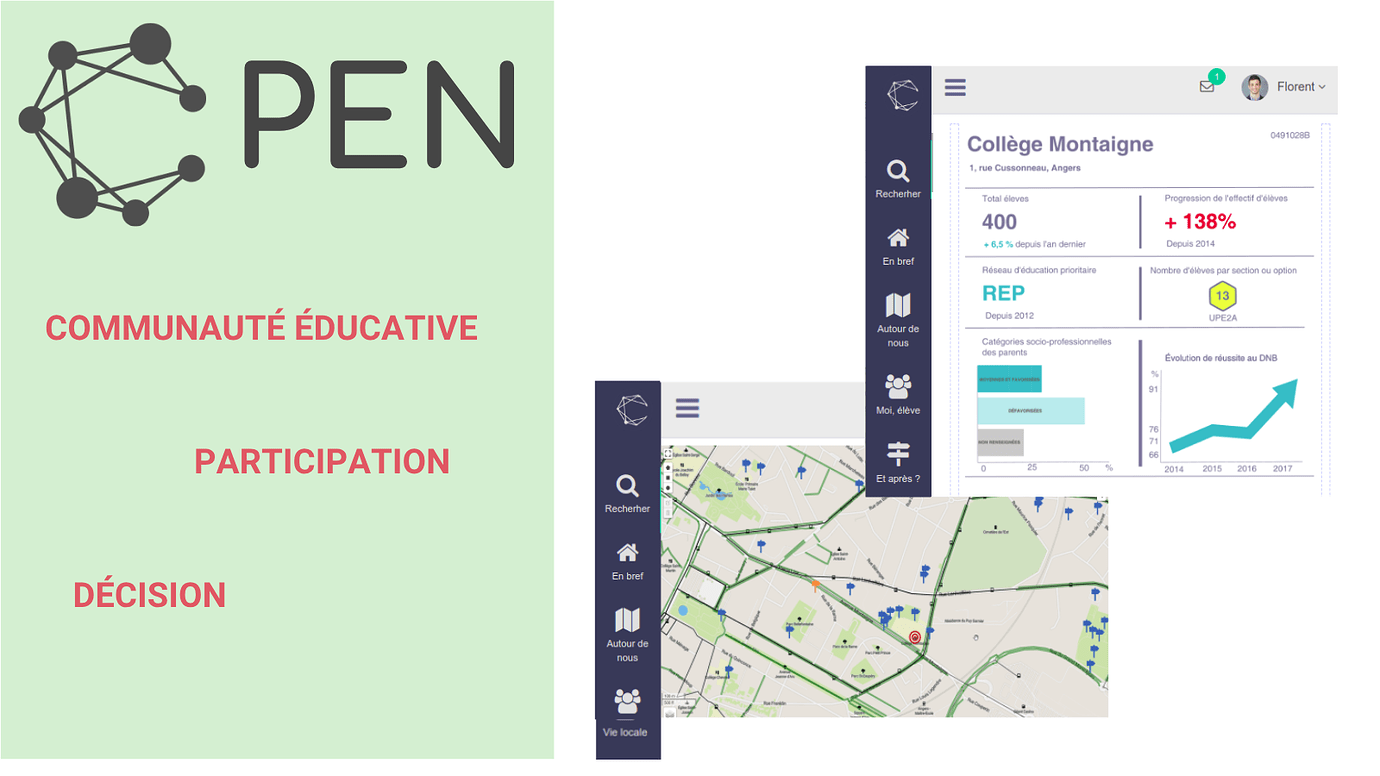
\includegraphics[width=0.7\linewidth]{./img/open} 

}

\caption{Visuels du service OPEN.}\label{fig:unnamed-chunk-9}
\end{figure}

\subsection{Antisèche}\label{antiseche}

\begin{quote}
\href{http://datavizchallenge.fr/t/dataviz-r-shinyapp/74}{Lien vers la
documentation}
\end{quote}

\textbf{Contexte : } Lors de leurs déplacements, les recteurs et agents
du ministère ont besoin d'accéder rapidement à une vue synthétique des
principales caractéristiques d'un établissement, où qu'ils soient et
sans avoir forcément accès à un poste informatique. Ils cherchent
également à pouvoir développer une vision comparative des informations
entre les établissements, afin de pouvoir orienter leur discours et
prise de décision.

Comment concevoir un outil répondant à l'ensemble de ces besoins ?

\textbf{Produit final}: Prototype d'application permettant une
visualisation géolocalisée des établissements, et d'accéder à une
présentation synthétique et ergonomique de leurs indicateurs principaux
(nombre d'élèves, taux de réussite au Brevet des Collèges, cours et
options proposées, capacité d'accueil, nombre d'enseignants par élève,
etc).

L'outil propose également une vision évolutive de ces indicateurs dans
le temps, ainsi qu'une fonction de filtrage permettant de cibler les
variables d'intérêt ¨

\begin{figure}

{\centering 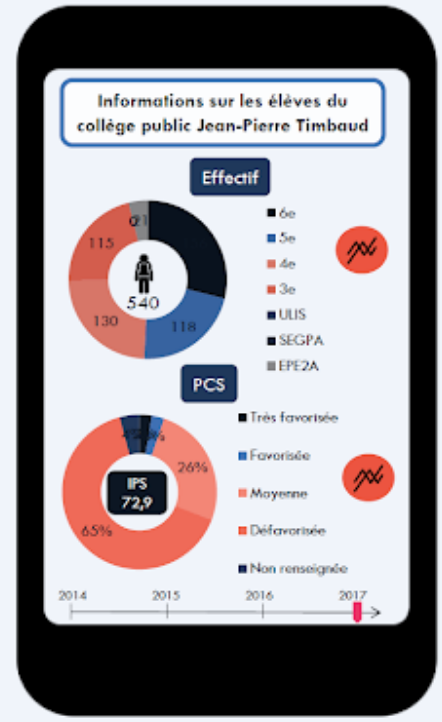
\includegraphics[width=0.4\linewidth]{./img/antiseche} 

}

\caption{Maquette du service Antisèche}\label{fig:unnamed-chunk-10}
\end{figure}

\section{Défi 3 : «Carto du numérique dans les
territoires»}\label{defi-3-carto-du-numerique-dans-les-territoires}

\subsection{Cadrage du défi}\label{cadrage-du-defi-2}

eCarto est un outil créé par la Caisse des Dépôts, en partenariat avec
le ministère de l'Education nationale et de la Jeunesse et les
associations de collectivités. Il permet de visualiser le déploiement du
numérique éducatif dans chacun des 63 000 établissements scolaires, en
rassemblant les données open data sur la connectivité, l'équipement, les
ressources et les expérimentations. Il a vocation à être un outil
permettant : * au plus grand nombre de s'informer sur l'état du
numérique éducatif en France ; * aux décideurs publics d'ajuster
l'accompagnement des académies et des collectivités en matière de
déploiement du numérique éducatif ; * aux acteurs des politiques
éducatives locales d'identifier plus facilement les établissements où un
enseignement à distance serait possible dans de bonnes conditions.

\textbf{Objectifs} : faciliter l'appropriation des données relatives au
déploiement du numérique éducatif en France en augmentant l'outil
eCarto.

\textbf{3 questions pour démarrer le DataViz Challenge :} * Quelles sont
les disparités territoriales observables ? * Quelles données
complémentaires et extensions possibles pour enrichir la représentation
du niveau de maturité numérique d'un territoire ? * Quelles mises en
perspective possibles entre niveau de maturité numérique et niveau
d'enclavement / isolement géographique d'un territoire ?

\subsection{🏆Alain Jette}\label{alain-jette}

\begin{quote}
\textbf{Projet retenu par le jury pour le défi 3}
\textbf{\href{https://drive.google.com/drive/folders/1dkZBb5xC6zCmAiD-EKUGl0TThzRDolEe}{Lien
vers la documentation}}
\end{quote}

\textbf{Contexte :}Les établissements scolaires regorgent de projets
pédagogiques. Cependant, ceux-ci ont souvent peu de visibilité au sein
de leur territoire, ce qui peut limiter leur portée et l'investissement
qu'ils reçoivent en ressources humaines, financières et matérielles
nécessaires à leur portage. Cette opacité peut également jouer sur
l'image d'un établissement, les indicateurs standards ne permettant pas
d'en valoriser la prise d'initiatives, la créativité et le dynamisme
internes.

Comment rendre visible les projets pédagogiques sur un territoire afin
de développer l'inspiration , le partenariat et l'action de tous ?

\textbf{Produit final}: Maquette de carte multidimensionnelle et
collaborative des projets pédagogiques. Son design inspiré de l'univers
de Lego invite à concevoir les projets pédagogiques comme des
co-constructions. L'outil recense l'ensemble des projets organisés sur
un territoire (ici l'Académie de Dijon) ainsi que leur description.

\begin{figure}

{\centering 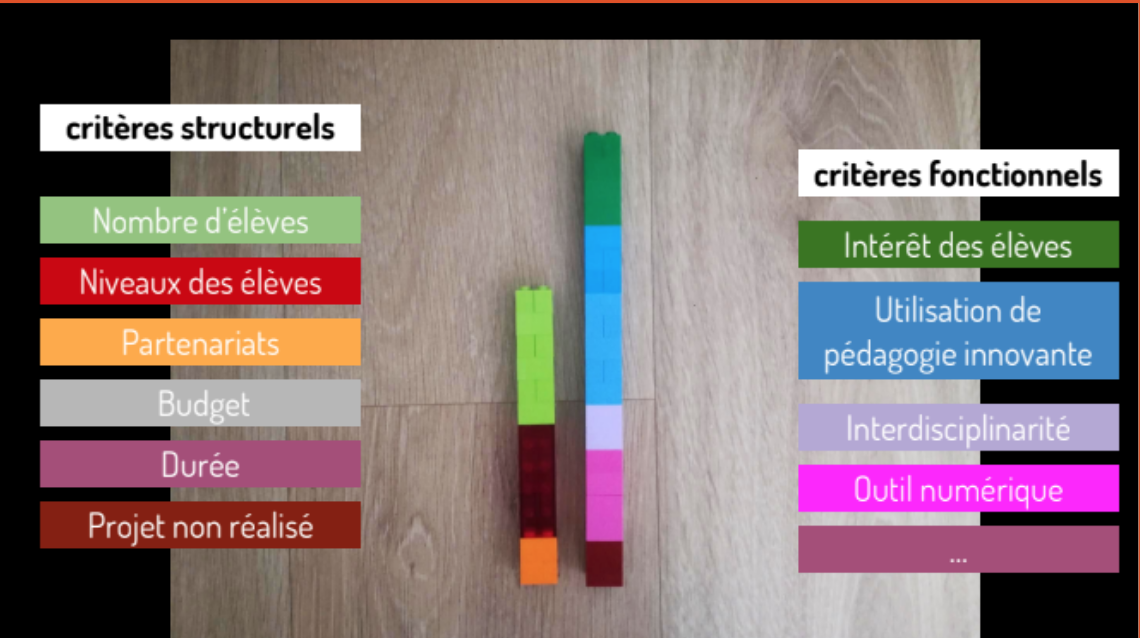
\includegraphics[width=0.7\linewidth]{./img/alainjette} 

}

\caption{Illustrations du projet à partir de LEGO.}\label{fig:unnamed-chunk-11}
\end{figure}

Il offre également un module de recherche ciblée selon des critères
structurels (nombre d'élèves, budget, durée, etc) et fonctionnels
(utilisation des outils numériques, pédagogie innovante,
interdisciplinarité, etc). Cette recherche affinée est amenée à
faciliter la conclusion de partenariats et le partage de ressources
entre les équipes pédagogiques, mais peut aussi aider le recteur à
piloter son académie. Cela permet finalement de valoriser aussi bien le
projet que son établissement d'accueil.

\subsection{Panser la fracture
numérique}\label{panser-la-fracture-numerique}

\begin{quote}
\href{https://drive.google.com/drive/folders/1dkZBb5xC6zCmAiD-EKUGl0TThzRDolEe}{Lien
vers la documentation}
\end{quote}

\textbf{Contexte} : Les établissements scolaires sont les premiers
touchés par les effets de la ``fracture numérique''. Ces inégalités ne
relèvent pas seulement de l'accès aux équipements informatiques, elles
sont également induites par d'autres paramètres tels que la couverture
numérique de l'établissement, sa catégorie (ex: REP/REP+), ses
financements, son nombre d'enseignants, leurs formations\ldots{}

Comment mesurer et visualiser les écarts de facilité d'accès au
numérique entre différents établissements en tenant compte de tous ces
paramètres pour mieux adapter les réponses politiques et évaluer leurs
impacts?

\textbf{Produit final} : Maquette de cartes en relief permettant de
visualiser un indicateur synthétique d'accès au numérique, d'en cibler
les composantes et de les comparer à ceux des établissements
environnants et à la moyenne nationale.

\begin{figure}

{\centering 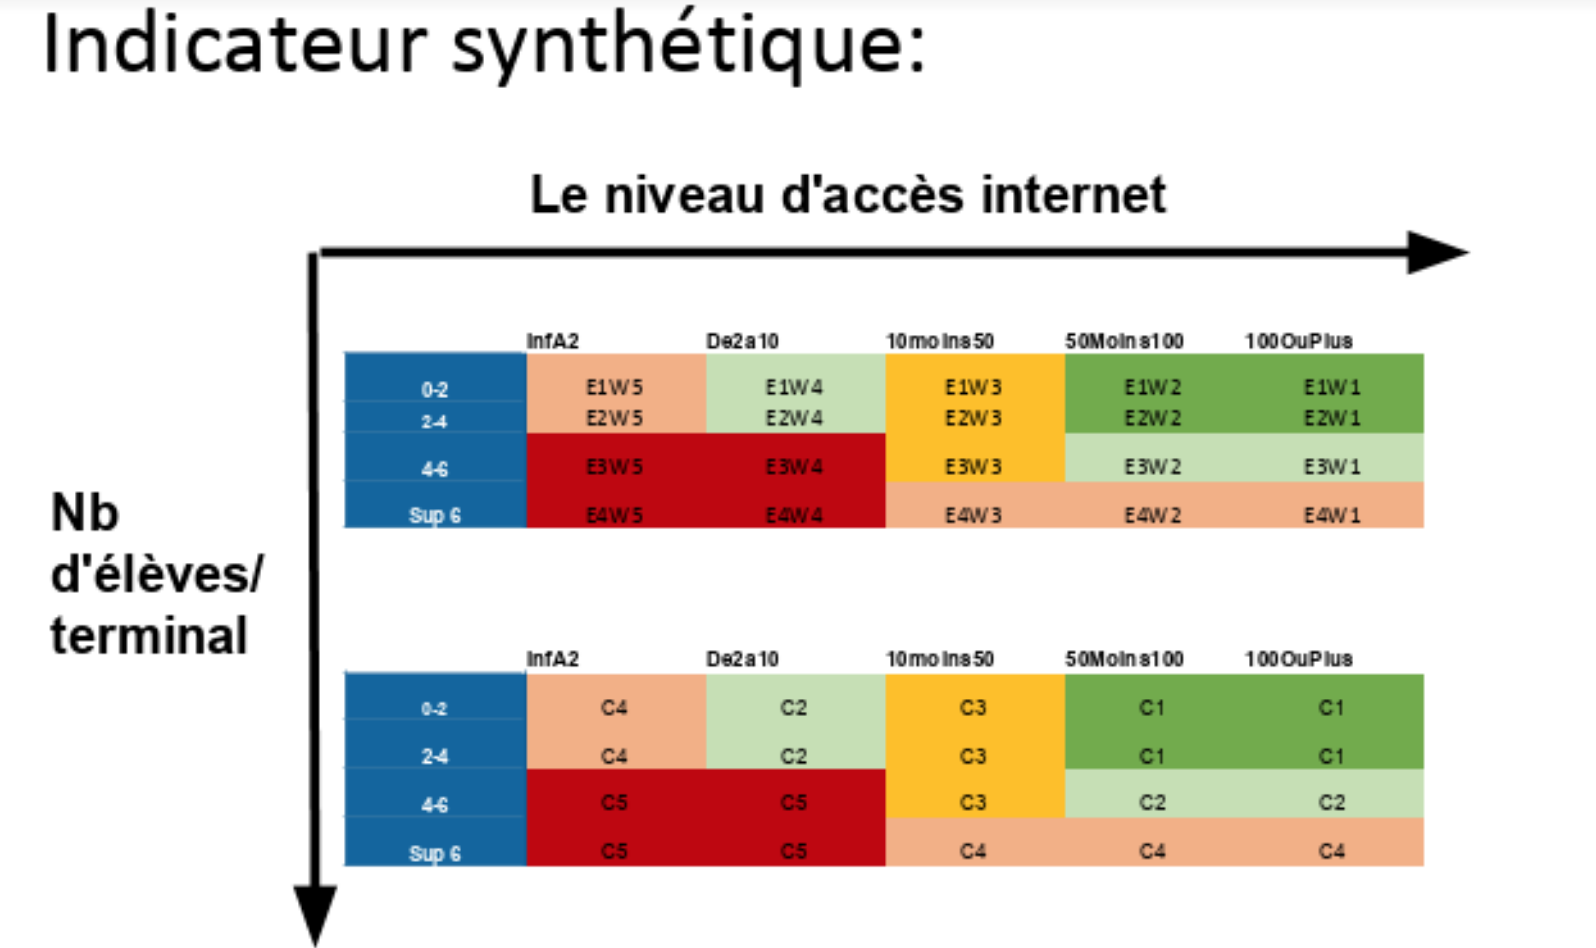
\includegraphics[width=0.7\linewidth]{./img/pan} 

}

\caption{Indicateur synthétique sur accès au numérique}\label{fig:unnamed-chunk-12}
\end{figure}

\textbf{Méthode} :

\begin{itemize}
\tightlist
\item
  Création d'un indicateur synthétique (Numeriscor) en croisant les
  données existantes (débit internet, nb d'élève/terminal, vétusté des
  équipements, etc) et d'autres données aujourd'hui difficilement
  trouvables (qualification des professeurs C2i2e, nombre de formations
  sur le numérique, etc)
\item
  intégration de l'indicateur à eCarto et à la fiche de chaque
  établissement.
\item
  création d'une moyenne départementale et nationale sur eCarto pour
  pouvoir facilement positionner un établissement par rapport aux autres
  et identifier ceux en difficultés
\end{itemize}

\chapter{Les principes d'un sprint data réussi}\label{principes}

\section{Au fait, c'est quoi un sprint data
?}\label{au-fait-cest-quoi-un-sprint-data}

Un sprint data, hackathon ou encore DataViz Challenge désigne tout
événement de durée variable pendant lesquel des personnes très diverses
se rassemblent pour résoudre des problèmes, classiquement en développant
des outils informatiques mais pas nécessairement. C'est un format de
co-création, associant sur un temps court (deux jours et une nuit dans
le cas du Dataviz Challenge) des profils et des compétences très
diverses au sein d'équipes projet, dans une ambiance de travail
conviviale, sous le signe de l'intelligence collective, du partage de
compétences et de connaissances.

Un sprint data combine 3 ingrédients essentiels :

\begin{itemize}
\item
  \textbf{des défis} qui sont des problèmes contextualisés que les
  participants devront résoudre en un temps limité ;
\item
  \textbf{des données} souvent ouvertes à l'occasion du sprint data qui
  constituent le matériau sur lequel les participants travaillent
\item
  \textbf{des participants} bénévoles qui dédient une partie de leur
  temps libre pour apprendre, partager leur connaissance, mettre les
  compétences au défi, s'entrainer sur de nouvelles données et
  rencontrer d'autres participants.
\end{itemize}

\section{Historique : du rite hacker de niche à la
prolifération}\label{historique-du-rite-hacker-de-niche-a-la-proliferation}

Historiquement, les sprint data répliquent un des rites des hackers, les
« marathons » de développement qui se déroulent pendant les conférences
des communautés issues du logiciel libre. Les concours de réutilisation
de données ouvertes sont aussi liés à l'émergence de deux concepts : le
\emph{crowdsourcing} qui considère que la participation massive (et
généralement bénévole) des internautes peut être une source majeure de
création de valeur voire de renouvellement de la démocratie et
\emph{l'innovation ouverte} qui consiste à diffuser une partie de
l'information stratégique à des acteurs extérieurs qui, par la mise en
compétition ou leur nombre, parviendront à mieux innover que les
ressources internes dont dispose l'organisation.

Dans le domaine des données ouvertes, Apps for Democracy a été un des
premiers concours de développement de services. Il s'est tenu à
Washington en 2008, quelques mois après le lancement de l'App Store
d'Apple et du développement de l'écosystème des applications mobiles.
Cet évènement a inspiré le développement de nombreux concours
d'applications notamment par la publication d'un guide qui a détaillé
pas à pas comment faire participer les développeurs à un concours
d'applications et a permis l'essaimage de ce modèle dans de nombreuses
villes.

\begin{figure}

{\centering 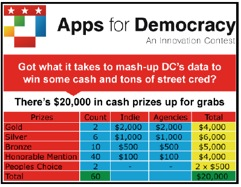
\includegraphics[width=0.3\linewidth]{./img/appsfordemocracycontest} 

}

\caption{Illustration du concours Apps for Democracy}\label{fig:unnamed-chunk-13}
\end{figure}

Depuis le premier concours de réutilisation de données ouvertes en
France à Rennes en 2010, les hackathons prolifèrent. Tous les principaux
ministères ont organisé un hackathon ces dernières années : le ministère
de l'intérieur dès 2014, \#HackRisques ou \#HackBioDiv pour
l'environnement, \#CodeImpot pour l'économie, Hackathon Marine pour la
défense, hackathon culture et tourisme\ldots{}

Cette prolifération de hackathons ou data sprint s'est accompagnée de
critiques grandissantes à l'égard du modèle. Bien que les participants à
un hackathon prennent sur leur temps personnel généralement le weekend,
certains organisateurs n'ont pas hésité à mettre trop de pression et
d'attentes sur les participant-e-s ce qui a pu dégrader l'expérience.
Aussi, la majorité des participant-e-s à un hackathon ne sont pas
rétribués ce qui a été dénoncé comme du travail déguisé sous l'allure
d'un évènement décontracté et informel. Des organisateurs ont, par
ailleurs, beaucoup valorisé le workaholism, une dépendance au travail
jusqu'à l'épuisement, en encourageant les participant-e-s à travailler
tout le weekend, toute la nuit, sans pause dans une compétition sans
arrêt. En réaction, le concept du
``\href{http://www.hackacon.fr/}{hackacon}'' parodie le hackathon en
développant des projets inutiles de manière ludique pendant un weekend
(voir \href{http://tracks.arte.tv/fr/hackacon}{reportage d'Arte}).

Un hackathon réussi se doit donc d'être bien préparé, convivial et pensé
comme une expérience enrichissante pour les participant-e-s.

\section{Les facteurs clés de succès}\label{les-facteurs-cles-de-succes}

\subsection{Mobiliser les parties prenantes internes et
externes}\label{mobiliser-les-parties-prenantes-internes-et-externes}

Simon Chignard dans
\href{https://donneesouvertes.info/2013/01/08/un-hackaton-sinon-rien/}{un
billet de blog} résume un hackathon en trois valeurs essentiels. La
première est la mobilisation, c'est souvent l'opportunité pour des
organisations d'enclencher une démarche d'open data en rencontrant
directement un public de réutilisateurs internes et externes pour les
jeux de données.

Comme l'explique
\href{http://www.internetactu.net/2012/11/16/les-dispositifs-creatifs-en-questions-22-les-limites-a-la-creativite-collective/}{Hubert
Guillaud dans InternetActu.net}, ces dispositifs créatifs transforment
l'approche traditionnelle de l'action publique : le côté très concret de
l'objectif (produire une application, un dispositif créatif, du code, un
objet\ldots{}) galvanise l'énergie. Stéphane Vincent, directeur de la
27e Région, explique dans ce même article que :

\begin{quote}
les dispositifs créatifs produisent ce que les organisations habituelles
n'arrivent pas à créer : un moment de décadrage, neutre et collectif,
totalement orienté vers la production de solutions ingénieuses. Ce sont
des formes joyeuses et non académiques de « recherche-action légère »,
qui permettent de conduire des micro-expériences dans des secteurs qui
en sont habituellement éloignés.
\end{quote}

Le sprint data permet ainsi d'avoir un nouveau regard sur les problèmes
qui rompt avec les habitudes du métier et de l'expérience. C'est
l'addition des compétences et des expertises qui produit un mélange
étonnant \textbf{fondé sur l'intelligence collective et le principe
selon lequel « le tout vaut plus que la somme des parties. »}

\subsection{Créer une expérience
stimulante}\label{creer-une-experience-stimulante}

La seconde valeur, c'est l'expérience : pour les participants,
l'excitation d'un hackathon peut être très stimulante. L'expérience du
hackathon casse les habitudes et sort de l'ordinaire, comme l'explique
Stéphane Vincent dans InternetActu.net :

\begin{quote}
A court terme, ce type de dispositifs transforme les participants
eux-mêmes, en particulier ceux directement concernés par les projets.
Ils se montrent souvent d'abord sceptiques (« Mais qu'est-ce que ces
gens peuvent bien connaître à mon domaine ? »), puis voient le
changement s'opérer. {[}\ldots{}{]}~Quand ces cessions sont bien menées,
elles font beaucoup plus que produire de l'innovation, elles produisent
du sens.
\end{quote}

Simon Chignard note que l'expérience du hackathon est conçue comme un
moment et un monde à part :

\begin{quote}
``l'unité de lieu (on vit en vase clos pendant 48 heures), le travail en
petit groupe d'individus qui ne se connaissaient pas nécessairement
auparavant (la colonie de vacances est l'archétype du team building,
c'est bien connu), la contrainte de temps (à la fin chaque groupe
présente son projet), voire la compétition (quand le hackathon donne
lieu à un vote).''
\end{quote}

Le problème c'est que cette expérience vécue est souvent mal restituée
par la suite, d'où l'importance de la documentation et de
l'accompagnement qui suivront.

\subsection{Créer une énergie
positive}\label{creer-une-energie-positive}

Pour Joshua Tauberer, organisateur d'Open Data Day DC et auteur de
\href{https://hackathon.guide/}{hackathon.guide}, un hackathon réussit
doit d'abord à l'énergie positive qu'il dégage. Les hackathons doivent
éviter de dériver vers une culture maladive de compétition et d'attentes
trop élevées sur les participant-e-s. Selon lui, le premier objectif
d'un hackathon doit être de renforcer une communauté tout en restant
ouvert à celles et ceux qui n'ont jusqu'alors pas ou peu utilisé de
données dans leur vie. On peut ainsi voir un hackathon comme une
occasion de découvrir et d'apprendre, que ce soit pour ses organisteurs
que pour ses participant-e-s.

En filigrane du Hackathon Guide, Joshua Tauberer pose la question de la
dimension compétitive du hackathon. La sélection de lauréats et la
remise de prix peuvent en effet attirer les meilleur-e-s et galvaniser
les participant-e-s mais elle peut aussi détériorer l'atmosphère et
créer une pression inutile. Il n'est pas indispensable de remettre des
prix aux meilleurs projets. Il faut en tout cas absolument éviter que la
sélection des lauréats donne l'impression aux participant-e-s qui n'ont
pas été sélectionnés d'être perdant ! On peut aussi envisager que tous
les participant-e-s repartent avec un prix ou une mention. Il faut donc
penser à valoriser le travail de tout le monde et à remercier
l'investissement de chacun.

La communication, la troisième valeur d'un sprint data selon Simon
Chignard, doit ainsi \textbf{ne pas céder aux sirènes de la
compétition}. Une organisation qui organise un sprint data doit aussi
selon
\href{https://www.regardscitoyens.org/apprenons-des-echecs-de-la-dila-episode-1-comment-faire-de-lopen-data/}{l'association
Regards Citoyens} ne pas trop se concentrer sur cette dimension
communicationnelle au détriment de l'ouverture et de la qualité des
données :

\begin{quote}
Si les données ont bien été libérées sous conditions Open Data, les
réutilisations arriveront sans doute d'elles-mêmes. Ne perdez pas donc
votre temps avant même l'ouverture à préparer des communications,
hackathons, sites officiels de réutilisation {[}\ldots{}{]} La tâche
d'ouverture est claire et balisée, le reste ne peut et ne doit venir
qu'ensuite !
\end{quote}

Maintenant que vous avez pris connaissance du contenu et des facteurs de
succès d'un sprint data, passons à la pratique et préparons notre
évènement !

\chapter{Les points d'attention dans la préparation du data
sprint}\label{preparation}

Les tâches dans l'organisation sont de plusieurs niveaux. Pour faciliter
l'organisation, mieux vaut se répartir la charge entre les différents
acteurs en charge de l'organisation du sprint data :

*le pilotage : certaines décisions devront être prises par la direction
ou l'organe de pilotage sur la supervision du chef de projet

\begin{itemize}
\item
  la communication : la mise en œuvre de certaines de ces tâches
  concernera essentiellement la direction de la communication
\item
  la logistique : ces tâches sont assurées principalement par le chef de
  projet et l'équipe présente lors de l'évènement
\item
  l'animation : ces tâches concernent principalement le chef de projet
  et l'animateur de l'évènement
\item
  post-évènement : ces tâches concernent le chef de projet et l'équipe
  présente lors de l'évènement.
\end{itemize}

Pour faciliter l'organisation d'un sprint data, nous mettons à
disposition un modèle de retroplanning qui liste les principales taches
à réaliser dans la préparation d'un sprint data. Il s'appuie sur les
bonnes pratiques internationales de l'organisation des hackathons et sur
l'expérience de l'association \href{okfn.fr}{Open Knowledge France}.
Certaines taches demanderont un travail plus ou moins considérable selon
les contraintes de l'équipe projet.

Pour utiliser le retroplanning pour votre propre évènement, rendez-vous
à
l'\href{https://docs.google.com/spreadsheets/d/13-deckO7z53tQu3dst0gQCh54HAmwPnMDfGiCLNax8M/edit?usp=sharing}{adresse
suivante} et créer une copie du document.

\begin{figure}

{\centering \includegraphics[width=0.6\linewidth]{./img/retroplanning} 

}

\caption{Le modèle de [retroplanning issu du dataviz challenge](https://docs.google.com/spreadsheets/d/13-deckO7z53tQu3dst0gQCh54HAmwPnMDfGiCLNax8M/edit?usp=sharing), les échéances ici reprennent la présentation du dataviz challenge.}\label{fig:unnamed-chunk-14}
\end{figure}

\subsection{La logistique}\label{la-logistique}

Repas Wifi Goodies

\subsection{La préparation des
données}\label{la-preparation-des-donnees}

Les obtenir le plus en amont possible Les faire expertiser par un
spécialiste

Datasheet for datasets

Cas des données confidentielles

\subsection{Le recrutement des participants et la mobilisation des
mentors}\label{le-recrutement-des-participants-et-la-mobilisation-des-mentors}

Communiquer tôt Demander des infos sur l'expérience data sprint et les
compétences

\subsection{La mise en place des espaces de discussion et de
documentation}\label{la-mise-en-place-des-espaces-de-discussion-et-de-documentation}

Présenter Discourse Digital Ocean Principales catégories du forum Le
package Vitrine

\subsection{La préparation du
programme}\label{la-preparation-du-programme}

Programme public

Conducteur :
\url{https://docs.google.com/spreadsheets/d/1x77Np6CK0f00M07VfUsjbQBRpW8SpClGe1s5jf6VYFw/edit\#gid=1858367361}

\chapter{L'animation du data sprint}\label{animation}

Matrice auto-évaluation :
\url{https://docs.google.com/presentation/d/1hTuVVXKd_NEwg26LZPuLaTX2KqDlz0S4BM824jacZak/edit\#slide=id.p}

Ice breaker

\section{Les trois temps créatifs : inspiration, idéation,
prototypage}\label{les-trois-temps-creatifs-inspiration-ideation-prototypage}

Même si chaque événement a ses particularités, on retrouvera dans le
DataViz Challenge les 3 temps du mouvement créatif.

\begin{figure}

{\centering 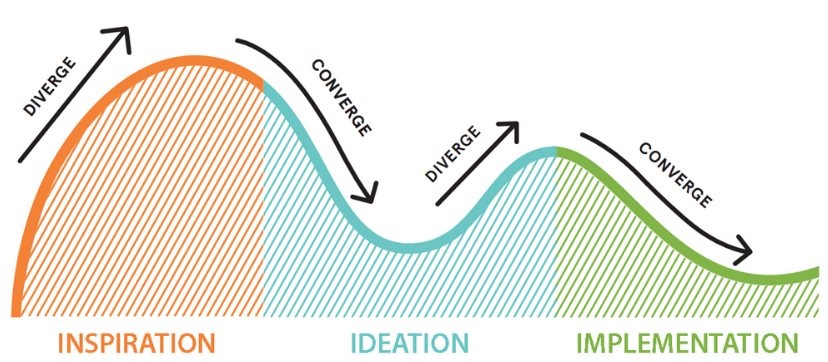
\includegraphics[width=0.7\linewidth]{./img/ideo} 

}

\caption{Les 3 temps du mouvement créatif (source : Danvang)}\label{fig:unnamed-chunk-15}
\end{figure}

\section{Inspiration : expliciter le contexte et les
défis}\label{inspiration-expliciter-le-contexte-et-les-defis}

Cette première phase vise à définir le problème et consiste à expliciter
les défis pour s'assurer qu'ils soient bien compris par les
participants. Le public doit pouvoir reformuler les défis proposés et
développer une compréhension partagée des enjeux.A quels problèmes
essayez-vous de répondre avec ce hackathon ? Pourquoi l'organisez vous ?
Qu'attendez-vous comme projet concret des participants ? Quels défis
sont proposés aux participants ?

Les défis en amont du hackathon sur le site de l'évènement et aussi
pendant le hackathon. Il est important de prendre ici une posture
d'empathie avec les participants pour s'assurer qu'ils comprennent et
adhèrent aux défis qui sont proposés. C'est une phase de divergence dans
laquelle le public doit pouvoir reformuler les défis proposés et dans
laquelle se développe une compréhension partagée des enjeux. Même si les
défis sont déjà formulés par écrit, il est important de prendre du temps
pour que les participants se l'approprient.

\textbf{Idéation} La seconde phase consiste à générer une multitude
d'idées autour du problème défini dans la phase précédente. Les
participants sont incités à explorer de nouvelles solutions aux défis
et, après un vote ou une phase de délibération, sélectionner les
propositions pour constituer un nombre limité d'équipes.

Quelles solutions peuvent répondre aux défis ? Comment les participants
envisagent de répondre à ces défis ? Cette phase de créativité se
déroule en deux temps : d'abord les participant-e-s doivent diverger en
livrant un maximum d'idées. Aucune idée ne doit être écartée, tout est
bon à prendre et chacun doit se sentir libre de faire part de ces
propositions. Des post-its suffiront à noter toutes les idées.

Il faut ensuite entrer dans une phase de convergence pour aboutir à des
équipes qui vont développer ensemble une solution. Pour cela, on peut
avoir recours à une étape de clustering pour rassembler les idées
similaires. Un bon moyen de former rapidement des équipes peut être
l'utilisation de gomettes : lors du dataviz challenge, nous avons
distribué une gomette à chaque participant-e. Chacun positionnait ses
deux gomettes sur les deux idées qui lui plaisaient le plus. A la suite,
nous avons utilisé deux grandes feuilles pour que chacun s'inscrive dans
les groupes projet qui avaient recueilli le plus de voix.

\textbf{Implémentation} Enfin, la troisième phase occupe la majeure
partie de l'événement puisque les participants prototypent, voire
développent, dans un temps limité, les visualisations de données ou
services qui tentent de répondre aux défis.

L'événement se terminera par l'attribution d'un prix à valeur
symbolique, pour valoriser les projets jugés les plus aboutis selon un
jury constitué d'experts de l'analyse de données ou de la thématique
traitée. Il n'y a pour autant pas de gagnants ni de perdants, cette
sélection sert surtout à donner de la visibilité aux projets les plus
emblématiques issus du data sprint.

\section{\texorpdfstring{Le ``off'' du sprint
data}{Le off du sprint data}}\label{le-off-du-sprint-data}

\subsection{Les ateliers de formation}\label{les-ateliers-de-formation}

\subsection{Les temps de pause et
d'inspiration}\label{les-temps-de-pause-et-dinspiration}

\subsection{La documentation des
projets}\label{la-documentation-des-projets}

\subsection{Quelques questions
logistiques}\label{quelques-questions-logistiques}

\chapter{La restitution et la suite}\label{restitution}

\section{Les présentations des
projets}\label{les-presentations-des-projets}

Le timing

Récupération des présentations

Demi-finale/finale ou finale en plenière ?

\section{La délibération du jury}\label{la-deliberation-du-jury}

Modèle Airtable :
\url{https://airtable.com/tbluLNQYV6eePmLw1/viwEFKUFYmTtF3SQ2?blocks=hide}

Fiche critères d'évaluation :
\url{https://docs.google.com/spreadsheets/d/1t_wpk0EityvplEkwQTYeQqbSN61RlNSRmkLtl58doxY/edit\#gid=0}

\section{La reprise de la
documentation}\label{la-reprise-de-la-documentation}

Contacter les participants Combler les manques dans la documentation
Raconter les projets de manière narrative

\section{Le sondage et le débriefing}\label{le-sondage-et-le-debriefing}

Modèle de questionnaire

Analyse du questionnaire, méthode DAKI

Faire une restitution publique :
\url{https://datafin.fr/enquete-sur-le-hackathon-datafin-de-juin-2018}

\section{L'accompagnement à donner}\label{laccompagnement-a-donner}

Présenter les résultats du projet à des décideurs Financer la suite

\bibliography{book.bib,packages.bib}


\end{document}
